\documentclass{report}
\usepackage[left=2cm,right=2cm,top=2cm,bottom=2cm,bindingoffset=0cm]{geometry}
\usepackage[utf8x]{inputenc}
\usepackage[english,russian]{babel}
\usepackage{amsfonts}
\usepackage{amsmath}
\usepackage{mathtools}

\usepackage{graphicx}
\graphicspath{{pictures/}}
\DeclareGraphicsExtensions{.pdf,.png,.jpg}

\begin{document}
\LARGE{ \textbf {Лекция 14 №}}\\
\Large{ \textbf {Пример дискретного отсечения}}\\
Нужной найти минимальное значение.
$z = 6x_1 + 4x_2 => min $\\
$2x_1 +x_2 => 3$\\
$x_1 - 2x_2 <= 2$\\
$x_1 , x_2$ - целые.\\

Канон\\
$-z = -6x_1 - 4x_2 => max(-z) $\\
$2x_1 +x_2 - x_3 = 3$\\
$x_1 - 2x_2 + x_4= 2$\\
$x_1 , x_2,x_3,x_4$ - целые.\\

Диаг\\
$-z = 6(-x_1) + 4(-x_2) => max(-z) $\\ все не то
$x_3 = -3 - 2(-x_1) +(-x_2) $\\
$x_4 =  2 +  (-x_1) -2(-x_2)= 2$\\
% $x_1 , x_2,x_3,x_4$ - целые.
Лексографический наименьший отрицательныйы элемент, \\
Для направляющего столбца коэффицент $u_2 = 1$
Для 2 столбца $u1 = [\frac{6}{4}] = 1$

Нормировка  производ строки, ищется для тех элементов производ строки, которые меньше 0.\\

$v_2 = - \frac{-1 = A_{32}}{u_2} = 1$

$v_1 = - \frac{-z = A_{31}}{u_1 = 1} = 2$
Выбираем максимальный.

Добавляем х5
Берется коэффицент производ строки, этот производ строка делется на  коэфицент этой строки $max = v_2 = 2$\\
Пишем наибольшее целое, не привышающее.

Дискретное отсечение и ведущий столбец, как направляющего.

Ведущий столбец на минус ведущий элемент, пишем его в новую таблицу.\\
$x_1 = \quad $ новый ведущий столбец на коэфицент из ведущий строки $-1$. Получившееся прибавить к этому столбцу.\\
Основная цель - сделать таблицу и прямо и двойственно допустимой.

2 шаг\\
Производ строка = с отрицательными элеменами.
Столбцы - с отрицательными числами, но лексографичиески наименьшие.\\

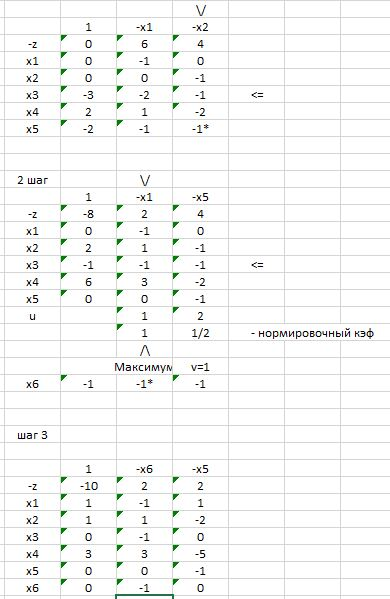
\includegraphics[width=\textwidth, height=\textheight]{4}


Ответ $z^* = 10, x_1 = 1, x_3=0, x_4 = 0$



\end{document}
